%todo: to describe the basic magic mirror idea, hardware and framework
%Magic Mirror framework: conception, software and hardware
\section{Magic Mirror Conception}
%the reason to choose anatomy learning for magic mirror conception
Knowledge about human anatomy is an important issue for everyone working in the field of medicine. But it is also an important part of the general education and it is relevant for many other professions related e.g. to health-care or sports. The human anatomy is very complex and it does not only involve knowledge about the single organ, but also about issues such as chemical processes, human motion and spatial relations inside the body. Therefore, teaching human anatomy is very difficult and often big effort is spent on teaching it e.g. by letting students perform dissection courses, creating illustrations and plastic models of anatomy or by utilizing 3D computer graphics.

The General Medical Council recently proposed standards for effective teaching and learning of medical students \cite{Council2009}. They stated that: ``...medical schools should take advantage of new technologies…. to deliver teaching.'' Augmented reality research has matured to a level that its applications can now be found in both mobile and non-mobile devices \cite{Bacca2014} and research on AR has also demonstrated its extreme usefulness for increasing student motivation in the learning process \cite{Chang2014,DiSerio2013}. Providing adequate learning experience to different learners is a challenging issue as the learning system generally does not adapt content to suit individual learner needs. Personalization for promoting a multimodal learning environment is also a growing area of interest, such as the development of user modeling and personalized processes which place the student at the center of the learning development.
\subsection{System}
A novel way to intuitively teach human anatomy using an augmented reality magic mirror system that displays anatomical structures overlaid onto the body of the user is presented. 
Our system prototype has a mirror-like effect to the user by projecting a ‘looking glass’ on the body. The prototype of the magic mirror is largely based on a software framework that has been developed for HMD-based AR. The system can currently display the skeleton of the user, rendered from pre-operative CT data. The mirror tracks users’ movements using a depth camera and an algorithm to detect the pose of the user from the depth image. This is realized using the Microsoft Kinect which was originally developed to allow controlling computer games by motion. By using the magic mirror metaphor, the user is led to believe that he or she is able to look inside their own body. At the same time, radiological information (CT, MRI data and a fully segmented dataset of cross-sectional photographs of the human body) are displayed in real-time. The user is able to select slices from these dataset by hand movement \cite{Blum2012,Navab2012a}.

The current system allows visualization of static anatomy on the user and offers a simple user interface to select CT, MR or photographic slices. Demos of the prototype have been given on various public occasions. This exposure to the public resulted in a several contacts with medical doctors (MD) from physiotherapy, anatomy, radiology, sports medicine, children’s medicine, and with medical teacher and science centers who are interested in using such a system in education of medical students and pupils. While discussions with these contacts were encouraging, most MDs asked for precision.
\subsubsection{Hardware setup}
\subsubsection{Software framework}
The interactive anatomy learning system which is presented in this paper is an augmented reality magic mirror and has primarily been developed for medical anatomy education, museums, and exhibitions. It focuses on bones and important organs of the thorax and abdomen. \figurename{\ref{fig:3-MMC:fingure1}} depicts the general view of the system, which includes a large display device and a Microsoft Kinect. The Microsoft Kinect contains both color and depth camera and is sold as an add-on for the Xbox 360 video game console, taking gestures, color image, body movement, and voice as game input. The user's skeleton and personal information can be generated from the Kinect sensor. The prototype of our magic mirror is largely based on a software framework that has been developed for HMD-based AR. Our system prototype has a mirror-like effect to the user by projecting a `looking glass' on the user body. The system can currently provide AR in-situ visualization, render skeleton from an original CT-volume, and showcase 3D models of organs.
\begin{figure}[ht]
	\centering
	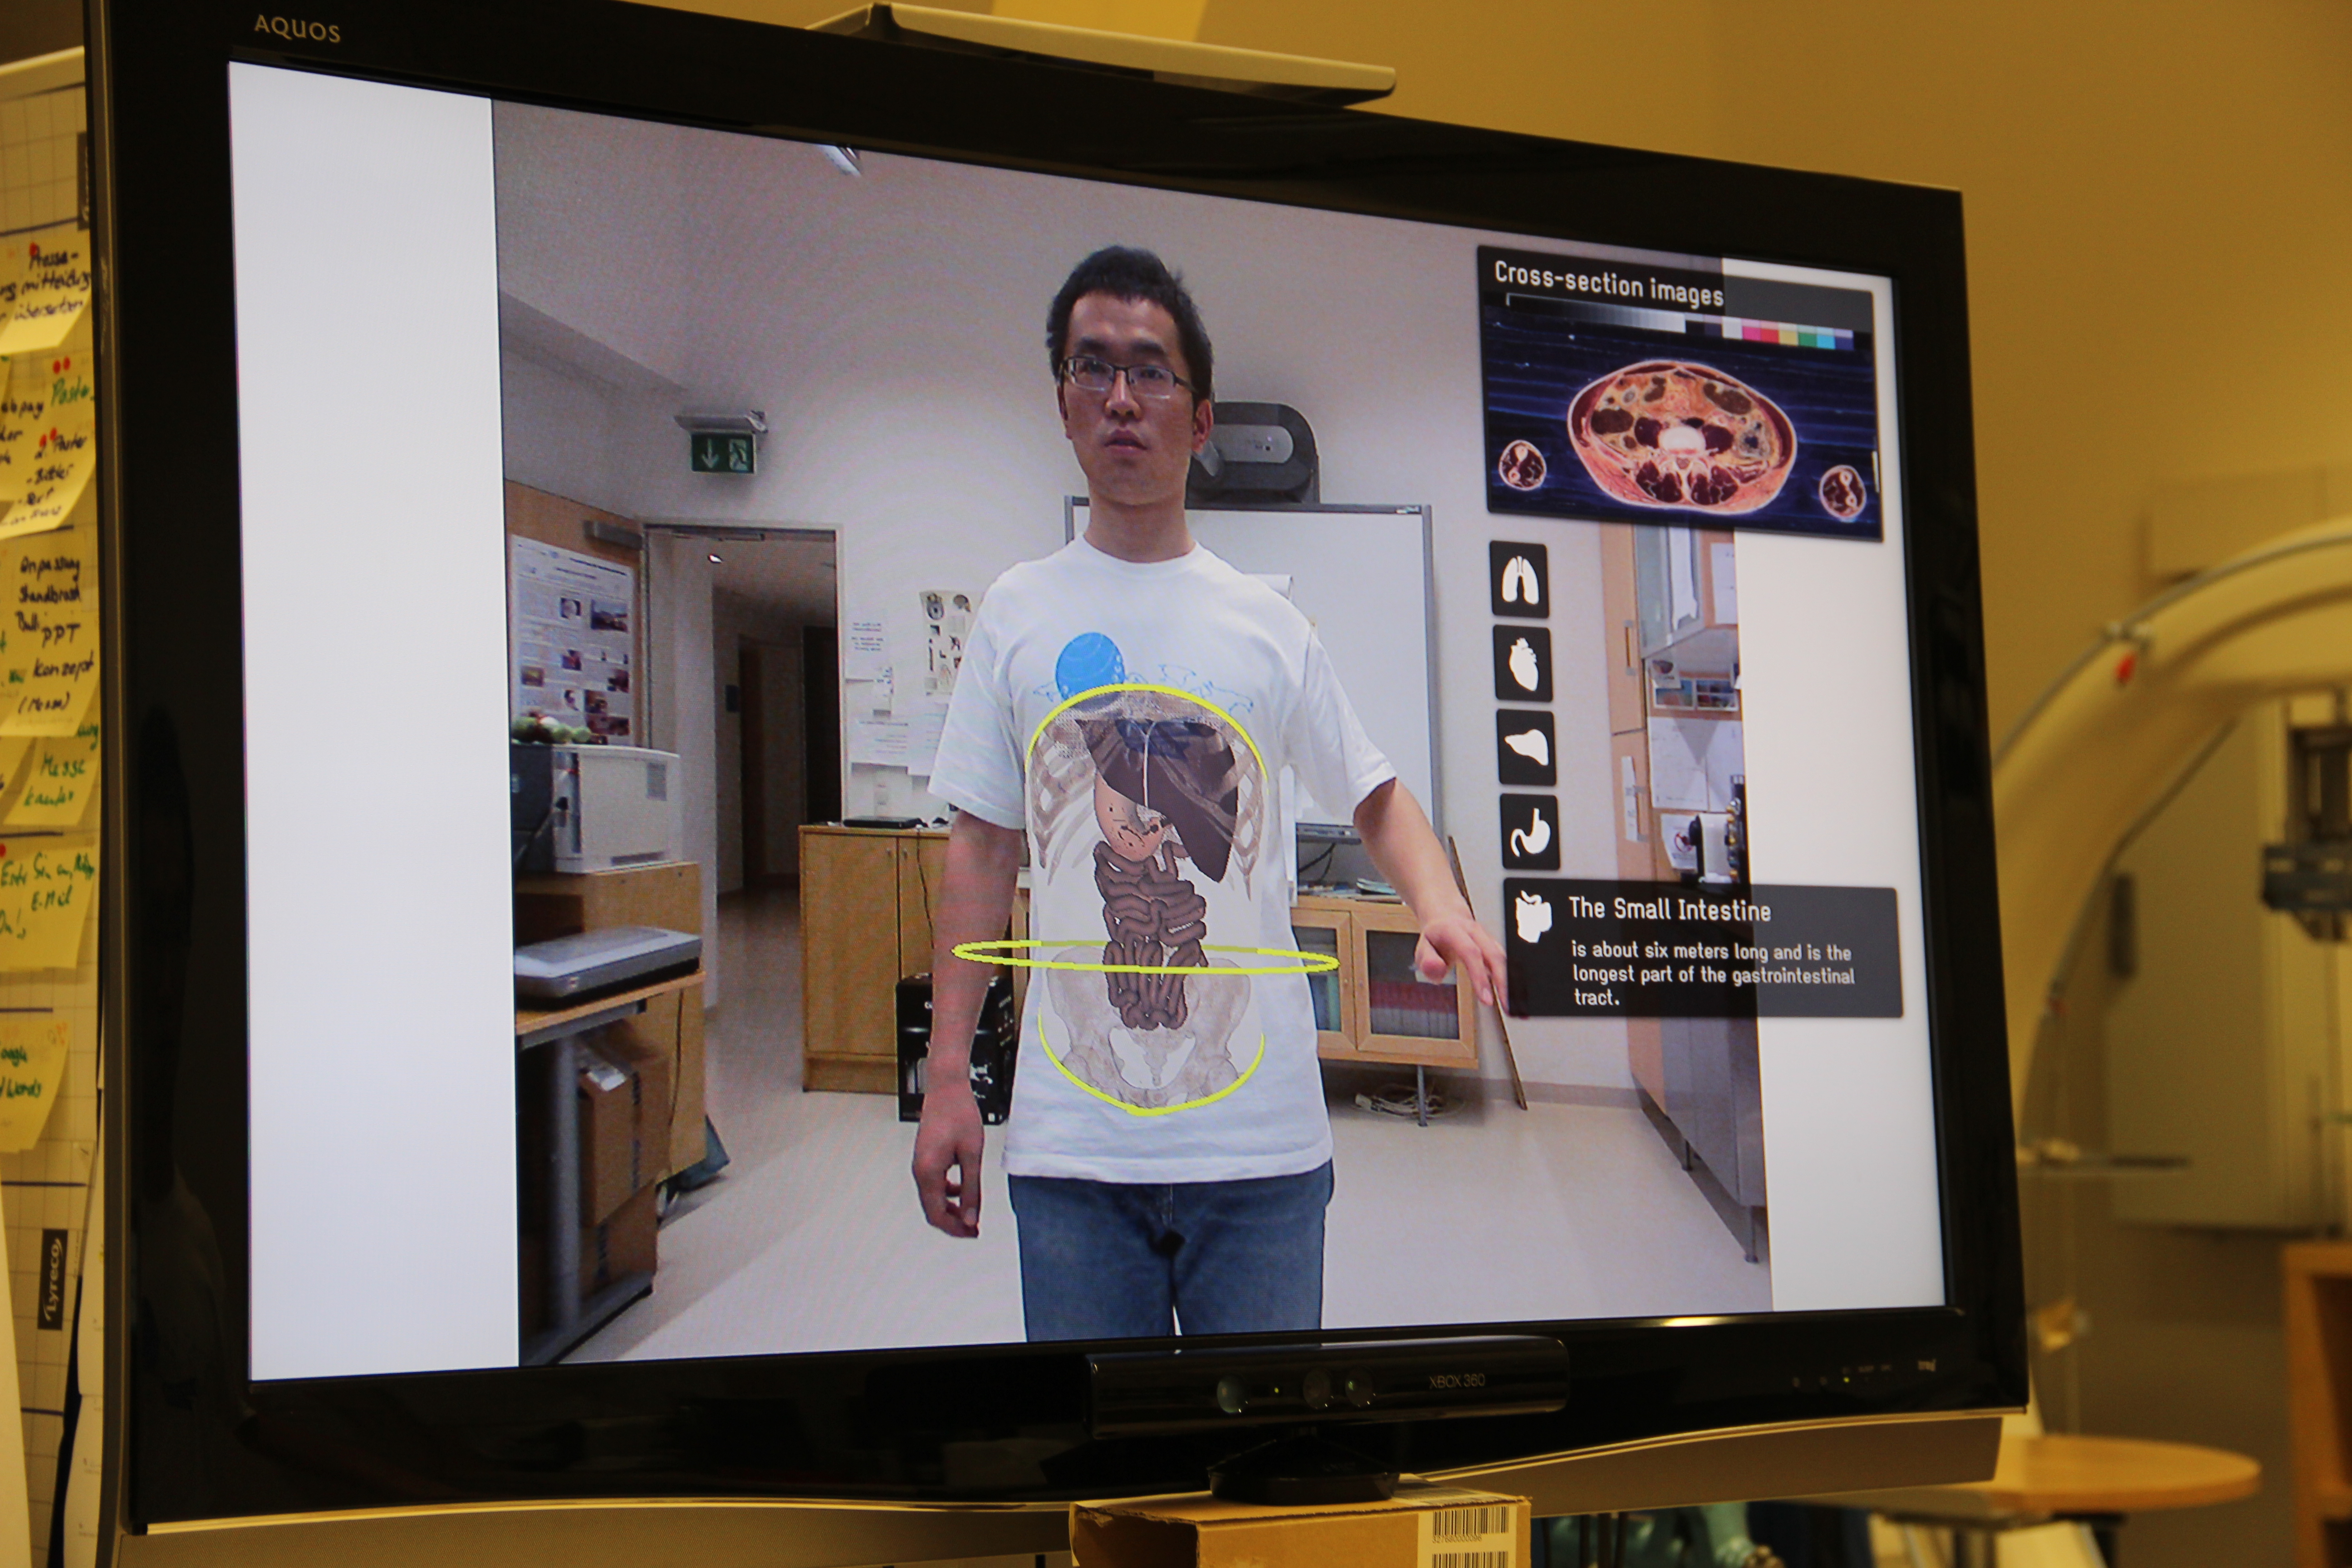
\includegraphics[width = 0.7\linewidth]{figures/3-MMC/Figure1.JPG}
	\label{fig:3-MMC:fingure1}
	\caption{Personalized magic mirror system for anatomy learning. A sensor tracks the user positions in real-time, and contextual in-situ visualization algorithms enable the augmentation of organs and muscles directly onto the user body.}
\end{figure}

\subsection{Natural perception and interaction}
\subsubsection{AR in-situ visualization of human anatomy}
For a personalized visualization of organs we employ the concept of a magic mirror. The camera image is flipped horizontally and shown on the screen such that the user has the impression of standing in front of a mirror. The system tracks all user movements using a depth camera and an algorithm to detect the pose of the user from the depth image. This is realized using the Microsoft Kinect which was originally developed to allow controlling computer games by motion. Then, virtual objects can be added to the image of the real scene. By using the magic mirror metaphor, the user is led to believe that he or she is able to look inside their own body. At the same time, radiological information (CT data and a fully segmented dataset of cross-sectional photographs of the human body) are displayed in real-time \cite{Blum2012}.

Prior to correctly using our AR magic mirror system, the users stand in front of the monitor and we displayed virtual marks near the five bone landmarks. The users are asked to interactively adjust the positions of the five marks to fit their own bone positions. In addition, the exact locations in the VKH CT dataset of the five selected bone landmarks are known. A linear interpolation was executed to estimate the torso point (i.e. a 6th landmark) in the CT volume to improve the overlay. Then the scale factors and transformation matrix were computed to render the anatomical image onto the user’s body. These landmark positions allow the deformation and interpolation of the medical data correctly within the magic mirror and onto the human body, resulting in a more precise augmentation. A user study involving surgeons and anatomy experts confirmed our findings and will be presented in Section 3.
\subsubsection{Natural User interaction}

\subsection{Potential application with magic mirror}
Medical education 
AR rehabilitation 
Patient positioning 
